\section{The Axiom of Completeness}
\begin{theorem}
	$\R$ contains $\Q$ as a subfield.
\end{theorem}
\begin{proof}
	Associate to each $q\in \Q$ the cut $q^* := \{r\in\Q : r<q\}$. Then the map $f:\Q \to \R$ with rule $q\mapsto q^*$ is an injection which preserves the field operations $+, \times$ and the order $<$. Then $\Q^*=\{q^*:q\in \Q\}$ is a subfield of $\R$.
\end{proof}
\begin{theorem}
	$\R$ satisfies the Axiom of Completeness.
\end{theorem}
\begin{proof}
	Let $A\subset \R$ be a collection of cuts with upper bound $\beta$. Let $\gamma = \bigcup_{\alpha\in A}A\subset \Q$. We first prove that $\gamma$ is a cut. $\gamma$ is trivially non-empty and not equal to $\Q$, because it must contain at least one cut, and because it is bounded by $\beta$ (and therefore properly contained in $\R$). Now, select some $p,q\in\alpha$, where $\alpha\in A$. If $q<p$, then $q\in\alpha$, and therefore $q\in\gamma$, so $\gamma$ is closed downwards. Now select $r\in\alpha$ such that $r>p$; it then follows that $r\in\gamma$ (since each $\alpha$ can not have a largest element). Hence, $\gamma$ is a Dedekind cut. \par
    Now, we show that $\sup A = \gamma$. Assume $\delta < \gamma$. Then there is an $s\in \gamma$ such that $s \not\in \delta$. Then $s$ must be contained in some $\alpha$, and thus $\delta < \alpha$. So, $\delta$ can not be an upper bound of $A$, and $\gamma = \sup A$ as a result.
\end{proof}

\begin{definition}
    The \emph{infimum} $\inf(S)=\alpha\in A$ of a set $S \subset A$ is a lower bound of $S$, where for $\beta > \alpha$, $\beta$ is not a lower bound for $S$.
\end{definition}

\begin{theorem}
	\emph{The Archimedean Property:} If $x,y \in \R$, with $x>0$, then there exists some $n\in\Z^+$ such that $nx>y$.
\end{theorem}
\begin{proof}
	Consider $A=\{nx:n\in\Z^+\}$. Let $y$ bound $A$. Then $A$ has a least upper bound $\sup A=\alpha$. It is clear that $\alpha - x$ is not an upper bound for $A$; so for some $m\in \Z^+$, $\alpha-x<mx$. But then $\alpha<mx+x=(m+1)x$, so $\alpha$ can not be an upper bound for $A$.
    \begin{center}
        
    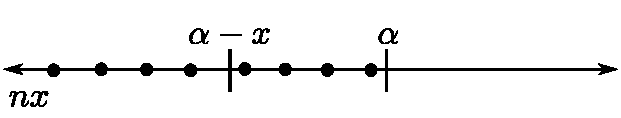
\includegraphics[width=.75\linewidth]{figures/archimideanpropertyproof.pdf}
    \captionof{figure}{$A$'s boundings.}

     \end{center}
\end{proof}

\begin{theorem}
	\emph{$\Q$ is dense in $\R$}: For each $x,y\in\R$, there is some $q\in\Q$ such that $x<q<y$.
\end{theorem}
\begin{proof}
	Choose $n$ such that $\frac{1}{n}<y-x$ (Archimedean property); consider multiples of $ \frac{1}{n}$, $\frac{m}{n}$, which grow without bound. Choose the least $\frac{m}{n}$ such that $\frac{m}{n}>x$. We want to show that $\frac{m}{n}<y$; claim the contrary. Then $\frac{m}{n}\geq y$ and $\frac{m-1}{x}<x$. But then $$-\frac{m-1}{n}>-x \Rightarrow -\frac{m-1+m}{n}=\frac{1}{n}>y-x,$$ a contradiction.
\end{proof}

\begin{theorem}
	\emph{Properties of suprema:} For $\gamma = \sup A$,
    \begin{enumerate}
	    \item $\gamma$ is an upper bound for some set $A$ if and only if $\sup A \leq \gamma$. 
        \item For all $a \in A$, $a \leq \gamma$, $\sup A \leq \gamma$.
        \item For all $a \in A$, $a < \gamma$, $\sup A \leq \gamma$.
        \item If $\gamma < \sup A$, then there exists an $a\in A$ such that $\gamma < a \leq \sup A$.
        \item If $A\subset B$, then $\sup A \leq \sup B$ (i.e., for all $a\in A$, $a\in B$, so $a \leq \sup B$). 
        \item To show that $\sup A = \sup B$, show that for all $a \in A$, there exists a $b\in B$ such that $a \leq b $, so $\sup A \leq \sup B$. A similar process applies to showing that $\sup B \in \sup A$, which proves equivalence.
	\end{enumerate}
\end{theorem}